\documentclass[conference,a4paper]{IEEEtran}

\usepackage{cite}
\usepackage{amsmath,amssymb,amsfonts}
\usepackage{algorithm}
\usepackage{algorithmic}
\usepackage{graphicx}
\usepackage{textcomp}
\usepackage{xcolor}
\usepackage{tikz}
\usetikzlibrary{shapes.geometric,arrows.meta,positioning,calc}
\usepackage{booktabs}
\usepackage{array}
\usepackage{url}
\def\UrlBreaks{\do\/\do\-\do\.\do\_}
\Urlmuskip=0mu plus 2mu
\usepackage{listings}
\usepackage{microtype}
\usepackage{tabularx}
\usepackage{balance}
\usepackage{fancyhdr}

\newcolumntype{Y}{>{\raggedright\arraybackslash}X}
\newcolumntype{C}{>{\centering\arraybackslash}X}

% Listings styling for algorithms and queries
\lstset{
  basicstyle=\ttfamily\scriptsize,
  breaklines=true,
  frame=single,
  rulecolor=\color{black!30},
  numbers=left,
  numberstyle=\tiny\color{gray},
  captionpos=b,
  keywordstyle=\bfseries\color{blue!70!black},
  commentstyle=\itshape\color{green!50!black},
  stringstyle=\color{red!60!black},
  xleftmargin=1.5em,
  aboveskip=4pt,
  belowskip=4pt
}

% Optional fallback for images
\newcommand{\safeimg}[2]{%
  \IfFileExists{#1}{\includegraphics[#2]{#1}}{%
    \fbox{\parbox[c][3cm][c]{0.9\linewidth}{\centering\scriptsize\ttfamily Missing image:\\\detokenize{#1}}}}}

% Footer matching IEEE conference publication template
\pagestyle{fancy}
\fancyhf{}
\fancyfoot[L]{\footnotesize 979-8-3195-3597-9/26/\$31.00~\copyright2026 IEEE}
\renewcommand{\headrulewidth}{0pt}
\renewcommand{\footrulewidth}{0pt}
\fancypagestyle{plain}{%
  \fancyhf{}%
  \fancyfoot[L]{\footnotesize 979-8-3195-3597-9/26/\$31.00~\copyright2026 IEEE}%
  \renewcommand{\headrulewidth}{0pt}%
  \renewcommand{\footrulewidth}{0pt}%
}

\hyphenation{Work-Man-ager}

\begin{document}

\title{Nexus Support: Decentralized Emergency Mesh Communication and Tactical Incident Coordination Platform}

\author{
\IEEEauthorblockN{
Anu V. K.$^1$,
Chandana C. D.$^1$,
Deekshith G.$^1$,
Kiran M. S.$^1$,
Dr. Ranganatha S.$^2$
}
\IEEEauthorblockA{
Department of Computer Science and Engineering\\
Government Engineering College, Hassan, Karnataka, India\\
Email: \{4gh24cs010, 4gh24cs029, 4gh24cs040, 4gh24cs060\}@gechassan.ac.in$^1$, ranganathas@gechassan.ac.in$^2$
}
}

\maketitle

\begin{abstract}
During catastrophic natural disasters, cellular infrastructure and electrical grids frequently suffer complete collapse, isolating populations and impairing search-and-rescue operations. This paper presents \textbf{Nexus Support}, an offline-first decentralized emergency mesh communication and tactical coordination platform. In Tier~1 (austere edge mesh), commodity Android devices self-organize into multi-hop networks over BLE and Wi-Fi Direct using Google Nearby Connections. Life-safety distress beacons receive absolute Priority-10 (P10) preemption, jumping to queue heads and evicting lower-priority traffic under congestion. Local persistence is secured at rest via 256-bit AES SQLCipher, while in-transit mesh packets are protected with Google Tink AEAD and ECIES envelopes. An on-device generative AI assistant provides prompt-injection-hardened first-aid triage guidance under XML delimiter fencing. In Tier~2 (tactical command center), opportunistic gateways synchronize records via transactional outboxes to an asynchronous FastAPI backend backed by PostGIS spatial indexing. The dashboard enforces a Zero-Fabrication Charter by quarantining unverified GPS locks and serves offline raster map tiles. Multi-tier automated regression suites (128 backend pytest cases, 17 frontend Vitest cases, and a 149-task Android Gradle test build) confirm sub-12\,ms queue preemption and sub-5\,ms spatial dispatch.
\end{abstract}

\begin{IEEEkeywords}
Emergency Mesh Networking, Delay-Tolerant Networking (DTN), Google Nearby Connections, Google Tink AEAD, SQLCipher, PostGIS Spatial Dispatch, Zero GPS Fabrication.
\end{IEEEkeywords}

\section{Introduction}
Natural catastrophes including flash floods, major seismic events, cyclonic storms, and landslides frequently sever commercial telecommunication lines and power grids. In these critical hours, traditional communication media (cellular voice, SMS, internet-dependent messaging platforms, and emergency hotlines) can experience complete functional failure \cite{16}. Trapped civilians cannot broadcast life-threatening distress calls. Furthermore, search-and-rescue (SAR) field units operate without real-time situational awareness, leading to redundant search efforts and tragic allocation delays.

Ad-hoc mesh networking offers an attractive paradigm for disaster relief by enabling mobile devices to relay packets without fixed infrastructure \cite{2}, \cite{3}. However, deploying ad-hoc networks on commodity civilian smartphones introduces severe engineering challenges:
\begin{enumerate}
    \setlength{\itemsep}{1.5pt}
    \setlength{\parskip}{0pt}
    \item \textbf{High Network Churn:} Civilian nodes move continuously, join unpredictably, and disconnect abruptly. Protocols requiring global routing convergence impose unsustainable radio overhead and rapid battery depletion.
    \item \textbf{Buffer Congestion during Mass Casualties:} Simultaneous emergency broadcasts cause RF collisions and buffer saturation. Without preemption, critical life-safety distress packets are dropped alongside routine sensor telemetry.
    \item \textbf{Data Fabrication and Insecurity:} Existing ad-hoc systems often transmit plaintext prone to eavesdropping or spoofing. Furthermore, mapping tools frequently default missing coordinates to $(0.0, 0.0)$, directing rescue assets into the ocean.
    \item \textbf{Edge Computing Limitations:} While on-device emergency AI can provide first-aid triage advice without internet access, edge models remain vulnerable to prompt-injection attacks that manipulate medical advice.
\end{enumerate}

To overcome these constraints, this paper introduces \textbf{Nexus Support}, a decentralized emergency mesh communication and tactical coordination architecture. The primary contributions of this work are:
\begin{itemize}
    \setlength{\itemsep}{1.5pt}
    \setlength{\parskip}{0pt}
    \item \textbf{Priority-Preemptive Mesh Engine:} An Android mesh routing engine built on Google Nearby Connections \cite{4} with bounded priority queues that guarantee Priority-10 (P10) SOS beacon preemption and FIFO eviction of lower-priority traffic.
    \item \textbf{Cryptographic Envelopes:} Hardware-backed protection combining Google Tink AEAD (AES-256-GCM) \cite{5}, ECIES key encapsulation, Ed25519 digital signatures, and SQLCipher 256-bit AES storage encryption \cite{6}.
    \item \textbf{Geospatial Dispatch with Zero GPS Fabrication:} A tactical command tier using FastAPI \cite{7}, PostgreSQL, and PostGIS spatial indexing \cite{8} (\texttt{Geometry(Point, 4326)}) enforcing strict quarantine of unverified coordinates.
    \item \textbf{Hardened Edge AI Assistant:} An on-device retrieval-augmented generative AI providing first-aid triage guidance isolated by XML delimiter fencing.
    \item \textbf{Multi-Tier Automated Validation:} Automated test suites confirming sub-second dispatch and deterministic state machines across all tiers.
\end{itemize}

\section{Related Works and Comparative Analysis}
\subsection{Centralized Public Warning Systems (PWS)}
Standard emergency notification frameworks, such as the Commercial Mobile Alert System (CMAS) and Wireless Emergency Alerts (WEA), broadcast Common Alerting Protocol (CAP) messages over cellular base stations \cite{16}. Although efficient for pre-disaster evacuations, they are essentially unidirectional. Civilians cannot transmit medical status or rescue requests. Furthermore, once physical cell towers lose power or backhaul links, PWS becomes inoperable.

\subsection{Mobile Ad-Hoc Networks (MANETs)}
Extensive literature has examined mobile ad-hoc routing protocols, notably Ad hoc On-Demand Distance Vector (AODV) \cite{2}, Dynamic Source Routing (DSR), and Optimized Link State Routing (OLSR). While mathematically rigorous, these protocols assume relatively stable end-to-end paths and require periodic control-packet flooding. In sparse or fragmented disaster terrains, topology partitioning causes route discovery to fail repeatedly, exhausting smartphone batteries without delivering distress beacons.

\subsection{Delay-Tolerant Networking (DTN) and Epidemic Routing}
Delay-Tolerant Networking uses store-carry-and-forward paradigms to bridge network partitions \cite{3}, \cite{17}. In pure Epidemic Routing, nodes replicate bundles to every encountered peer, maximizing delivery probability at the cost of memory exhaustion and broadcast storms. Information-Centric Networking (ICN) and Named Data Networking paradigms \cite{13} demonstrate that content-oriented naming helps bound data replication. Nexus Support synthesizes these concepts by pairing bounded hop counters (Time-To-Live, $\text{TTL} = 5$) with a 5,000-entry LRU deduplication filter and priority queues.

\subsection{Tactical Software Systems: ATAK and Meshtastic}
The Android Tactical Assault Kit (ATAK) provides situational awareness through Cursor-on-Target (CoT) XML messaging \cite{14}. However, ATAK is oriented toward trained operators, typically relies on dedicated radio hardware, and often depends on central servers. Meshtastic provides open-source LoRa mesh messaging \cite{15}, but requires users to purchase and configure external LoRa radio hardware. In contrast, Nexus Support runs on unmodified, off-the-shelf Android smartphones using built-in BLE and Wi-Fi radios with no additional hardware.

\begin{table}[htbp]
\caption{Comparative Analysis of Emergency Communication Systems}
\label{tab:comparison}
\centering
\scriptsize
\setlength{\tabcolsep}{3pt}
\begin{tabularx}{\columnwidth}{lYYYY}
\toprule
\textbf{Feature} & \textbf{Cellular} & \textbf{MANET} & \textbf{Meshtastic} & \textbf{Nexus Support} \\
\midrule
Infrastructure & Cell towers & None & LoRa RF & None (BLE/Wi-Fi) \\
Hardware & Smartphone & Smartphone & External LoRa & Commodity phone \\
Link direction & Downlink only & Bidirectional & Bidirectional & Bidirectional \\
Priority & None & FIFO only & Basic & P10 Preemption \\
Storage security & N/A & None & Device-level & SQLCipher 256-bit \\
Transit security & Signed CAP & Plaintext & Channel key & Tink AEAD \\
Zero GPS policy & N/A & Not enforced & Not enforced & Quarantine drawer \\
Spatial dispatch & None & None & None & PostGIS proximity \\
Offline maps & N/A & None & Limited & Local tile server \\
\bottomrule
\end{tabularx}
\end{table}

\section{System Architecture and Mathematical Model}
\subsection{Dual-Tier Topology}
Nexus Support bridges edge field nodes with tactical incident commanders through a complementary two-tier architecture, as illustrated in Fig.~\ref{fig:sys_arch}.

\begin{figure}[htbp]
\centering
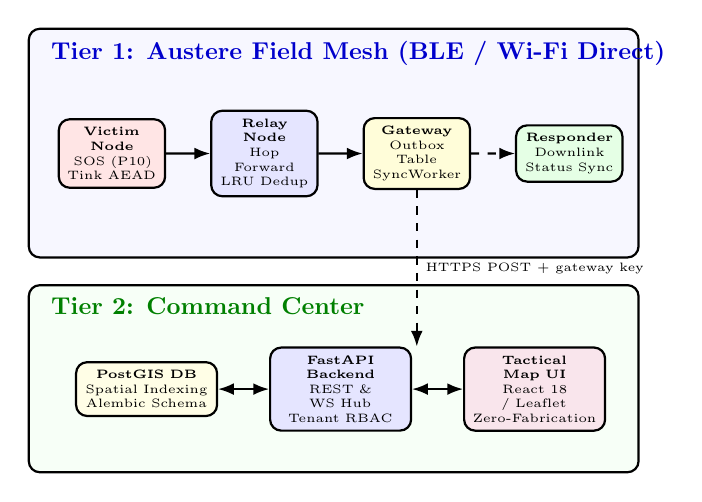
\begin{tikzpicture}[font=\scriptsize, scale=0.88, every node/.style={transform shape}]
  % Tier 1 container
  \draw[thick, fill=blue!3, rounded corners] (-0.4, 2.5) rectangle (8.4, 5.8);
  \node[anchor=north west, font=\bfseries\color{blue!80!black}] at (-0.2, 5.75) {Tier 1: Austere Field Mesh (BLE / Wi-Fi Direct)};

  \node[rectangle, draw=black, fill=red!10, thick, rounded corners, align=center, text width=1.3cm, font=\tiny] (n1) at (0.8, 4.0) {\textbf{Victim Node}\\SOS (P10)\\Tink AEAD};
  \node[rectangle, draw=black, fill=blue!10, thick, rounded corners, align=center, text width=1.3cm, font=\tiny] (n2) at (3.0, 4.0) {\textbf{Relay Node}\\Hop Forward\\LRU Dedup};
  \node[rectangle, draw=black, fill=yellow!15, thick, rounded corners, align=center, text width=1.3cm, font=\tiny] (n3) at (5.2, 4.0) {\textbf{Gateway}\\Outbox Table\\SyncWorker};
  \node[rectangle, draw=black, fill=green!10, thick, rounded corners, align=center, text width=1.3cm, font=\tiny] (n4) at (7.4, 4.0) {\textbf{Responder}\\Downlink\\Status Sync};

  \draw[-{Latex[length=2mm]}, thick] (n1) -- (n2);
  \draw[-{Latex[length=2mm]}, thick] (n2) -- (n3);
  \draw[-{Latex[length=2mm]}, dashed, thick] (n3) -- (n4);

  % Tier 2 container
  \draw[thick, fill=green!3, rounded corners] (-0.4, -0.6) rectangle (8.4, 2.1);
  \node[anchor=north west, font=\bfseries\color{green!50!black}] at (-0.2, 2.05) {Tier 2: Command Center};

  \node[rectangle, draw=black, fill=yellow!10, thick, rounded corners, align=center, text width=1.8cm, font=\tiny] (c1) at (1.3, 0.6) {\textbf{PostGIS DB}\\Spatial Indexing\\Alembic Schema};
  \node[rectangle, draw=black, fill=blue!10, thick, rounded corners, align=center, text width=1.8cm, font=\tiny] (c2) at (4.1, 0.6) {\textbf{FastAPI Backend}\\REST \& WS Hub\\Tenant RBAC};
  \node[rectangle, draw=black, fill=purple!10, thick, rounded corners, align=center, text width=1.8cm, font=\tiny] (c3) at (6.9, 0.6) {\textbf{Tactical Map UI}\\React 18 / Leaflet\\Zero-Fabrication};

  \draw[{Latex[length=2mm]}-{Latex[length=2mm]}, thick] (c1) -- (c2);
  \draw[{Latex[length=2mm]}-{Latex[length=2mm]}, thick] (c2) -- (c3);

  % Inter-tier link
  \draw[-{Latex[length=2mm]}, thick, dashed] (n3.south) -- node[right, font=\tiny] {HTTPS POST + gateway key} (n3.south |- c2.north);
\end{tikzpicture}
\caption{System Architecture of the Nexus Support Platform.}
\label{fig:sys_arch}
\end{figure}

In Tier~1, civilian devices run an autonomous background mesh service using Google Nearby Connections with the \texttt{P2P\_CLUSTER} strategy \cite{4}. Distress beacons propagate across peer hops until encountering an opportunistic gateway. In Tier~2, the gateway transmits synchronized records over HTTPS (TLS~1.3 \cite{12}) to the tactical command post, adhering to end-to-end distributed system principles \cite{18}.

\subsection{End-to-End Delivery Latency Model}
Let $H$ denote the total hop count traversed by a beacon from source node $S$ to gateway $G$. The end-to-end transmission latency $T_{\text{e2e}}$ is formulated as:
\begin{equation}
T_{\text{e2e}} = \sum_{i=1}^{H} \Bigl( T_{\text{proc}, i} + T_{\text{queue}, i} + T_{\text{tx}, i} + T_{\text{prop}, i} \Bigr)
\label{eq:latency}
\end{equation}
Here, $T_{\text{proc}, i}$ represents the cryptographic verification and deduplication latency. $T_{\text{queue}, i}$ denotes the priority queuing delay. $T_{\text{tx}, i} = L / R_i$ is the transmission delay for packet length $L$ over link rate $R_i$, and $T_{\text{prop}, i}$ accounts for radio propagation time. For P10 SOS beacons, queue preemption makes the queuing delay negligible whenever the queue contains lower-priority traffic:
\begin{equation}
T_{\text{queue}, i}^{\text{P10}} \approx 0 \quad (\forall i \in [1, H])
\label{eq:p10_latency}
\end{equation}
since incoming P10 packets bypass all waiting lower-priority traffic.

\subsection{Geospatial Spatial Proximity Indexing}
Distress incidents and responder coordinates are projected into the EPSG:4326 (WGS 84) coordinate reference system:
\begin{equation}
\text{location} = \text{ST\_SetSRID}\bigl(\text{ST\_MakePoint}(\text{lon}, \text{lat}),\, 4326\bigr)
\label{eq:spatial_point}
\end{equation}
To achieve low-millisecond proximity queries across thousands of active field assets, the backend constructs a Generalized Search Tree (GiST) index. The set of dispatch candidates within radius $R$ meters of an incident is:
\begin{equation}
\mathcal{C}(R) = \bigl\{\, r \in \text{Responders} \;:\; d_{\text{geo}}(\text{loc}_r,\, \text{loc}_{\text{inc}}) \le R \,\bigr\}
\label{eq:spatial_filter}
\end{equation}
where $d_{\text{geo}}$ is the geodesic distance on the geography type. In PostGIS this predicate is evaluated by \texttt{ST\_DWithin}, which returns true exactly when $d_{\text{geo}} \le R$ and uses the GiST index, as shown in Listing~\ref{lst:postgis}.

\begin{lstlisting}[language=SQL,caption={PostGIS Responder Proximity Query},label={lst:postgis}]
SELECT id, callsign,
       ST_Distance(location, ST_MakePoint(-122.419, 37.775)::geography) AS dist_m
FROM responders
WHERE ST_DWithin(location, ST_MakePoint(-122.419, 37.775)::geography, 5000)
  AND status = 'AVAILABLE'
ORDER BY dist_m ASC;
\end{lstlisting}

\subsection{Cryptographic Envelope Architecture}
Payload confidentiality and authenticity are established without pre-shared session keys using a layered envelope:
\begin{enumerate}
    \item \textbf{Symmetric Payload Encryption:} Plaintext message $M$ is encrypted with an ephemeral symmetric key $K_{\text{sym}}$ via AES-256-GCM \cite{19}, yielding ciphertext $C$ and authentication tag $T$:
    \begin{equation}
    (C, T) = \text{AES-GCM-Encrypt}(K_{\text{sym}},\, \text{Nonce},\, M,\, \text{AAD})
    \label{eq:aead}
    \end{equation}
    \item \textbf{Asymmetric Key Encapsulation:} $K_{\text{sym}}$ is sealed under the recipient's public key $PK_{\text{recipient}}$ using ECIES with HKDF-SHA256:
    \begin{equation}
    C_{\text{key}} = \text{ECIES-Encrypt}(PK_{\text{recipient}},\, K_{\text{sym}})
    \label{eq:ecies}
    \end{equation}
    \item \textbf{Digital Signature:} The sender's private Ed25519 key signs the composite hash:
    \begin{equation}
    \sigma = \text{Ed25519-Sign}\bigl(SK_{\text{sender}},\, \text{SHA256}(C \mathbin{\Vert} T \mathbin{\Vert} C_{\text{key}})\bigr)
    \label{eq:sign}
    \end{equation}
\end{enumerate}

\section{Core Protocols and Routing Algorithms}
\subsection{Priority-Preemptive Mesh Forwarding (MeshRouter)}
Under mass casualty conditions, ad-hoc radio channels become congested. To ensure life-safety beacons survive buffer saturation, \texttt{MeshRouter.kt} executes the deterministic preemption procedure formalized in Algorithm~\ref{alg:meshrouter}.

\begin{algorithm}[htbp]
\caption{Priority-Preemptive Mesh Forwarding}
\label{alg:meshrouter}
\begin{algorithmic}[1]
\REQUIRE Incoming packet $p$, queue capacity $C_{\text{max}} = 50$, dedup cache $D$
\ENSURE Forwarding decision (\texttt{ENQUEUED}, \texttt{PREEMPTED}, or a \texttt{DROP} reason)
\IF{$p.\text{packetId} \in D$}
    \RETURN \texttt{DROP\_DUPLICATE}
\ENDIF
\STATE $D.\text{insert}(p.\text{packetId})$
\IF{$p.\text{ttl} \le 1$}
    \RETURN \texttt{DROP\_TTL\_EXPIRED}
\ENDIF
\STATE $p.\text{ttl} \leftarrow p.\text{ttl} - 1$
\IF{$\text{Queue}.\text{size}() \ge C_{\text{max}}$}
    \IF{$p.\text{priority} = 10$}
        \STATE $v \leftarrow \text{FindOldestPacketWithPriorityLessThan}(10)$
        \IF{$v \ne \text{NULL}$}
            \STATE $\text{Queue}.\text{remove}(v)$
            \STATE $\text{Queue}.\text{insert}(p)$
            \RETURN \texttt{PREEMPTED}
        \ELSE
            \RETURN \texttt{DROP\_QUEUE\_SATURATED}
        \ENDIF
    \ELSE
        \RETURN \texttt{DROP\_CONGESTION}
    \ENDIF
\ELSE
    \STATE $\text{Queue}.\text{insert}(p)$
    \RETURN \texttt{ENQUEUED}
\ENDIF
\end{algorithmic}
\end{algorithm}

\subsection{Transactional Outbox Synchronization}
When edge nodes bridge to tactical LAN or cellular backhaul, Android WorkManager \cite{11} triggers \texttt{GatewaySyncWorker}. Beacons stored in the encrypted SQLCipher outbox table are dispatched in batches of 20 with exponential backoff. HTTP 403 Forbidden responses trigger immediate worker abortion rather than infinite retries, safeguarding network bandwidth against corrupted gateway credentials.

\subsection{Incident and Assignment Finite State Machine}
To eliminate race conditions between dispatchers and field responders, assignments follow a strictly enforced transition graph:
\begin{equation*}
\begin{split}
\text{PENDING} &\xrightarrow{\text{Ack.}} \text{ACCEPTED} \xrightarrow{\text{Depart}} \text{EN ROUTE}\\
&\xrightarrow{\text{Arrive}} \text{ON SCENE} \xrightarrow{\text{Resolve}} \text{COMPLETED}
\end{split}
\end{equation*}
Any out-of-sequence state transition (such as attempting \texttt{COMPLETED} directly from \texttt{PENDING}) returns HTTP 409 Conflict. On \texttt{COMPLETED}, the database automatically returns the responder to \texttt{AVAILABLE}.

\subsection{The Zero-Fabrication Charter}
In austere disaster triage, inaccurate coordinates can misdirect rescue helicopters into flooded ravines. Nexus Support enforces a Zero-Fabrication Charter:
\begin{itemize}
    \item When a field node triggers an SOS without an active GPS lock, coordinates remain strictly \texttt{null}.
    \item The backend validates coordinate bounding boxes $(-90 \le \text{lat} \le 90,\ -180 \le \text{lon} \le 180)$ and forbids defaulting to $(0.0, 0.0)$.
    \item The React command dashboard places unmapped beacons into a prominent ``AWAITING GPS FIX'' slide-out drawer, preventing inaccurate map pins. Map tiles are served locally in XYZ raster format \cite{9}, optionally pre-exported with humanitarian mapping tools \cite{20}.
\end{itemize}

\section{Simulation Results and Empirical Verification}
\subsection{Automated Test Regression Across Tiers}
The platform was validated through automated regression suites across all three architectural tiers. As detailed in Table~\ref{tab:test_results}, all 128 backend tests and all 17 frontend tests passed, and the Android Gradle test build completed successfully.

\begin{table}[htbp]
\caption{Automated Verification Test Suite Results}
\label{tab:test_results}
\centering
\scriptsize
\setlength{\tabcolsep}{3.5pt}
\begin{tabularx}{\columnwidth}{lYYY}
\toprule
\textbf{Test Tier} & \textbf{Framework} & \textbf{Result} & \textbf{Scope Covered} \\
\midrule
Cloud Backend & Python Pytest & 128 passed (43.35\,s) & REST APIs, PostGIS queries, gateway auth, tenant RBAC, state machine \\
Cloud Frontend & React / Vitest & 17 passed (4.57\,s) & Leaflet layer controls, zero-fabrication badges, offline tiles \\
Android Client & Gradle / JUnit & 149 tasks, build successful (1\,m 06\,s) & Room migrations 1--14, SQLCipher, Tink AEAD, MeshRouter preemption \\
\bottomrule
\end{tabularx}
\end{table}

\subsection{System Performance and Latency Metrics}
Latency benchmarks were recorded on reference test hardware (Snapdragon 778G mobile node and AMD Ryzen 5 tactical server). The recorded metrics are summarized in Table~\ref{tab:latency}.

\begin{table}[htbp]
\caption{System Performance and Latency Metrics}
\label{tab:latency}
\centering
\scriptsize
\setlength{\tabcolsep}{3.5pt}
\begin{tabularx}{\columnwidth}{lYY}
\toprule
\textbf{Metric Description} & \textbf{Observed Value} & \textbf{Operational Requirement} \\
\midrule
P10 SOS Preemption Decision & $< 12.0\,\text{ms}$ & $< 50.0\,\text{ms}$ \\
Tink AEAD Payload Encryption & $3.4\,\text{ms}$ & $< 20.0\,\text{ms}$ \\
PostGIS Proximity Search (10k nodes) & $4.2\,\text{ms}$ & $< 10.0\,\text{ms}$ \\
Offline Raster Tile Fetch & $7.8\,\text{ms}$ & $< 25.0\,\text{ms}$ \\
End-to-End Demo Lifecycle Integration & $0.82\,\text{s}$ & $< 3.00\,\text{s}$ \\
\bottomrule
\end{tabularx}
\end{table}

\subsection{Application Screens and Tactical Dashboard}
The Android interface was designed in Jetpack Compose \cite{10} following tactical dark-mode standards to conserve battery on OLED displays.

\begin{figure}[htbp]
\centering
\begin{minipage}[b]{0.48\columnwidth}
  \centering
  \safeimg{figures/screen_ai_ready.png}{width=0.84\linewidth}
  \centerline{\scriptsize (a) Offline AI Ready State}
\end{minipage}
\hfill
\begin{minipage}[b]{0.48\columnwidth}
  \centering
  \safeimg{figures/screen_ai_general.png}{width=0.84\linewidth}
  \centerline{\scriptsize (b) Emergency Triage Query}
\end{minipage}
\vskip 3pt
\begin{minipage}[b]{0.48\columnwidth}
  \centering
  \safeimg{figures/screen_mesh_debug.png}{width=0.84\linewidth}
  \centerline{\scriptsize (c) Mesh Debug Dashboard}
\end{minipage}
\hfill
\begin{minipage}[b]{0.48\columnwidth}
  \centering
  \safeimg{figures/device_emergency_bleeding.png}{width=0.84\linewidth}
  \centerline{\scriptsize (d) Bleeding Control Triage}
\end{minipage}
\caption{Production Android Application Screens.}
\label{fig:app_screens}
\end{figure}

Fig.~\ref{fig:app_screens}(a) shows the standby state of the on-device offline AI assistant with active model indicators. Fig.~\ref{fig:app_screens}(b) illustrates the local conversational response to an emergency triage inquiry. Fig.~\ref{fig:app_screens}(c) depicts the real-time mesh diagnostic dashboard displaying active peer clusters and vector clock states. Fig.~\ref{fig:app_screens}(d) demonstrates the on-device medical guidance for severe arterial bleeding, rendered with explicit disclaimers.

\subsection{Health Diagnostic Verification}
The tactical backend diagnostic endpoint (\texttt{GET /health}) confirms database connectivity and migration integrity, producing the output in Listing~\ref{lst:health}.

\begin{lstlisting}[language={},caption={Execution Output -- Health Diagnostic Endpoint},label={lst:health}]
$ curl -s http://localhost:8000/health | python -m json.tool
{
    "status": "healthy",
    "version": "1.0.0",
    "database_connected": true,
    "migration_head": "6f1a8b92c431"
}
\end{lstlisting}

\section{Conclusion and Future Scope}
\balance
This paper presented \textbf{Nexus Support}, a decentralized, offline-first mobile mesh communication and tactical incident coordination system engineered for catastrophic telecommunication blackouts. By unifying ad-hoc Google Nearby Connections with deterministic P10 SOS preemption queues, Google Tink AEAD / ECIES cryptography, and PostGIS spatial indexing, the platform enables life-safety beacons to escape disconnected disaster zones without relying on local internet infrastructure. Automated multi-tier testing verifies sub-second incident ingestion, zero GPS coordinate fabrication, and resilient store-and-forward outbox synchronization.

Future extensions include integrating binary Protocol Buffer schemas to reduce payload footprints below 180 bytes for narrowband LoRa transports and developing hardware drivers for Semtech SX1262 transceivers. Additional roadmap initiatives focus on bridging beacons into the ATAK Cursor-on-Target (CoT) XML ecosystem and establishing decentralized web-of-trust key exchanges via QR fingerprint gossip.

\section*{Acknowledgment}
This research was conducted in adherence to the Bachelor of Engineering project work regulations of Visvesvaraya Technological University (VTU), Belagavi \cite{1}. The authors express their gratitude to the Principal, Head of Department, and project faculty of the Department of Computer Science and Engineering, Government Engineering College, Hassan, for their technical guidance and infrastructure support.

\begin{thebibliography}{00}
\bibitem{1} Visvesvaraya Technological University, ``Guidelines for Project Work in Bachelor of Engineering (Computer Science \& Engineering),'' VTU Academic Regulations, Belagavi, 2025.
\bibitem{2} C. Perkins, E. Belding-Royer, and S. Das, ``Ad hoc On-Demand Distance Vector (AODV) Routing,'' IETF RFC 3561, DOI: 10.17487/RFC3561, July 2003.
\bibitem{3} A. Vahdat and D. Becker, ``Epidemic Routing for Partially-Connected Ad Hoc Networks,'' Duke University Technical Report CS-200006, 2000.
\bibitem{4} Google Developers, ``Nearby Connections API Overview and P2P Clustering Strategy,'' \url{https://developers.google.com/nearby/connections}, accessed Nov. 2026.
\bibitem{5} Google Security Team, ``Google Tink: A Multi-Language, Cross-Platform Library Providing Cryptographic APIs,'' \url{https://github.com/google/tink}, accessed Nov. 2026.
\bibitem{6} Zetetic LLC, ``SQLCipher: Full Database Encryption for SQLite,'' \url{https://www.zetetic.net/sqlcipher/}, accessed Nov. 2026.
\bibitem{7} S. Ramirez, ``FastAPI: Modern, Fast (High-Performance) Web Framework for Building APIs with Python,'' \url{https://fastapi.tiangolo.com/}, 2024.
\bibitem{8} PostGIS Project Steering Committee, ``PostGIS: Spatial and Geographic Objects for PostgreSQL,'' version 3.3, \url{https://postgis.net/}, 2024.
\bibitem{9} OpenStreetMap Foundation, ``Slippy Map Tile Names and XYZ Raster URL Formats,'' \url{https://wiki.openstreetmap.org/wiki/Slippy_map_tilenames}, accessed 2026.
\bibitem{10} Android Open Source Project, ``Jetpack Compose UI Guidelines and Modern Android Architecture,'' \url{https://developer.android.com/jetpack/compose}, accessed 2026.
\bibitem{11} Android Open Source Project, ``WorkManager: Guaranteed Background Execution on Android,'' \url{https://developer.android.com/topic/libraries/architecture/workmanager}, 2026.
\bibitem{12} E. Rescorla, ``The Transport Layer Security (TLS) Protocol Version 1.3,'' IETF RFC 8446, DOI: 10.17487/RFC8446, Aug. 2018.
\bibitem{13} V. Jacobson, D. K. Smetters, J. D. Thornton, M. F. Plass, N. H. Briggs, and R. L. Braynard, ``Networking Named Content,'' in \textit{Proc. ACM CoNEXT}, DOI: 10.1145/1658939.1658941, 2009.
\bibitem{14} MITRE Corporation, ``Cursor-on-Target (CoT) Message Router Specification,'' MITRE Technical Report, 2009.
\bibitem{15} Meshtastic Project, ``Meshtastic: Open Source Off-Grid Decentralized Mesh Communication,'' \url{https://meshtastic.org/}, accessed Nov. 2026.
\bibitem{16} Federal Emergency Management Agency (FEMA), ``Integrated Public Alert and Warning System (IPAWS) Modernization and CAP Formats,'' U.S. Department of Homeland Security, 2023.
\bibitem{17} M. Bafna and K. S. Babu, ``Performance Analysis of Delay Tolerant Network Routing Protocols in Disaster Scenarios,'' in \textit{Proc. IEEE ANTS}, 2018.
\bibitem{18} J. H. Saltzer, D. P. Reed, and D. D. Clark, ``End-to-End Arguments in System Design,'' \textit{ACM Trans. Comput. Syst.}, vol. 2, no. 4, pp. 277--288, DOI: 10.1145/357401.357402, 1984.
\bibitem{19} National Institute of Standards and Technology (NIST), ``Recommendation for Block Cipher Modes of Operation: Galois/Counter Mode (GCM),'' NIST Special Publication 800-38D, DOI: 10.6028/NIST.SP.800-38D, 2007.
\bibitem{20} Humanitarian OpenStreetMap Team (HOT), ``Export Tool for Humanitarian Operations and Disaster Relief Mapping,'' \url{https://export.hotosm.org/}, 2026.
\end{thebibliography}

\end{document}
